\documentclass{beamer}
\usetheme{Madrid}
\usecolortheme{default}

% Additional packages
\usepackage{graphicx}
\usepackage{amsmath}
\usepackage{listings}
\usepackage{xcolor}
\usepackage{subcaption}
\usepackage{tikz}
\usepackage{pgfplots}
\pgfplotsset{compat=1.15}

% Custom colors and styles
\definecolor{codegreen}{rgb}{0,0.6,0}
\definecolor{codegray}{rgb}{0.5,0.5,0.5}
\definecolor{backcolour}{rgb}{0.95,0.95,0.92}

\lstdefinestyle{mystyle}{
    backgroundcolor=\color{backcolour},   
    commentstyle=\color{codegreen},
    basicstyle=\ttfamily\small,
    breakatwhitespace=false,         
    breaklines=true,                 
    keepspaces=true,                 
    showspaces=false,                
    showstringspaces=false,
    showtabs=false,                  
    tabsize=2
}
\lstset{style=mystyle}

% Handle missing images gracefully
\DeclareGraphicsExtensions{.pdf,.png,.jpg}

% Add the results directory to the graphics path
\graphicspath{{../../results/}}

\title{Neural Implicit Flow: A Comparative Study}
\subtitle{Implementation Approaches and Performance Analysis}
\author{Christian Beneke}
\date{10.02.2025}

\begin{document}

\begin{frame}
    \titlepage
\end{frame}

\begin{frame}{Outline}
    \tableofcontents
\end{frame}

\section{Introduction}
\begin{frame}{Problem Space \& Motivation}
    \begin{itemize}
        \item High-dimensional spatio-temporal dynamics are computationally challenging
        \item Traditional methods face limitations:
        \begin{itemize}
            \item Fixed mesh structures (SVD, CAE)
            \item Poor scaling with high-dimensional data
            \item Limited ability to capture nonlinear dynamics
        \end{itemize}
        \item Real-world applications require:
        \begin{itemize}
            \item Adaptive mesh handling
            \item Efficient dimensionality reduction
            \item Real-time processing capabilities
        \end{itemize}
    \end{itemize}
\end{frame}

% \begin{frame}{Key Challenges in Current Approaches}
%     \begin{itemize}
%         \item Singular Value Decomposition (SVD)
%         \begin{itemize}
%             \item Limited to fixed mesh structures
%             \item Poor scaling with dimensionality
%         \end{itemize}
%         \item Convolutional Autoencoders (CAE)
%         \begin{itemize}
%             \item Requires uniform grid resolution
%             \item Struggles with adaptive meshing
%         \end{itemize}
%         \item Common Issues
%         \begin{itemize}
%             \item High computational overhead
%             \item Limited expressiveness for complex dynamics
%             \item Poor generalization to new scenarios
%         \end{itemize}
%     \end{itemize}
% \end{frame}

\section{Neural Implicit Flow Framework}
\begin{frame}{Core Architecture}
    \begin{columns}
        \column{0.5\textwidth}
        Two specialized networks:
        \begin{itemize}
            \item ShapeNet: Spatial complexity
            \item ParameterNet: Temporal evolution
        \end{itemize}

        \column{0.5\textwidth}
        Key innovations:
        \begin{itemize}
            \item Mesh-agnostic representation
            \item Efficient parameter sharing
            \item Adaptive complexity handling
        \end{itemize}        
    \end{columns}
    \begin{figure}
        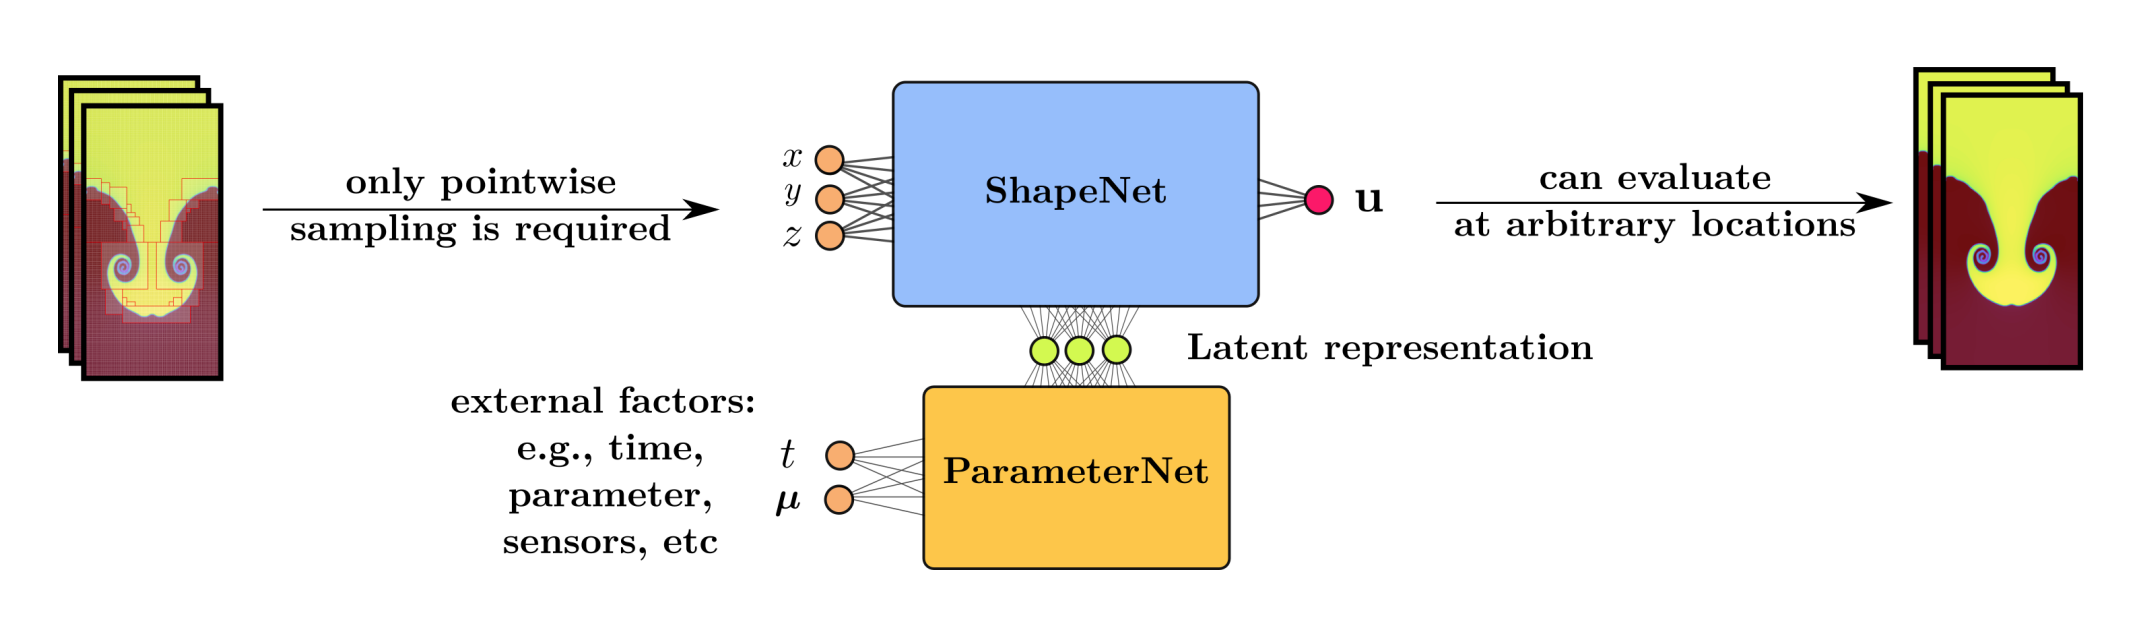
\includegraphics[width=\textwidth]{../../20-minute-presentation/latex/hypernetwork_diagram}
        \caption{NIF Architecture}
    \end{figure}
\end{frame}

\begin{frame}{Mathematical Formulation}
    \begin{itemize}
        \item Core mapping function:
        \[ f_\theta: (\mathbf{x}, \mathbf{t}) \mapsto u(\mathbf{x}, \mathbf{t}) \]
        where:
        \begin{itemize}
            \item $\mathbf{x} \in \mathbb{R}^d, d \in \mathbb{N}$: Spatial coordinate
            \item $\mathbf{t} \in \mathbb{R}^p, p \in \mathbb{N}$: Temporal/parametric input
        \end{itemize}
        \item Hypernetwork decomposition:
        \[ f_\theta(\mathbf{x}, \mathbf{t}) = \text{ShapeNet}_{\text{ParameterNet}_{\theta_p}(\mathbf{t})}(\mathbf{x}) \]
    \end{itemize}
\end{frame}

\section{Implementation Approaches}
\begin{frame}{Implementation Overview}
    \begin{itemize}
        \item Three distinct implementations:
        \begin{itemize}
            \item Upstream Reference (TensorFlow)
            \item TensorFlow Functional API
            \item PyTorch Implementation
        \end{itemize}
        \item Key considerations:
        \begin{itemize}
            \item Framework-specific optimizations
            \item Code maintainability
        \end{itemize}
    \end{itemize}
\end{frame}

\section{Experimental Setup}
\begin{frame}{Common Setup}
    \begin{itemize}
        \item Implemented base class for common functionality
        \item Implemented two of the given example cases
        \item Made optimiser configurable (Adam, AdaBelief)
        \item Comprehensive training logger with visualization
    \end{itemize}
\end{frame}

\begin{frame}{Upstream Reference Implementation}
    \begin{itemize}
        \item Based on original paper implementation
        \item Key modifications:
        \begin{itemize}
            \item Migration to current TensorFlow version
            \item Various bug fixes needed to run the provided examples
        \end{itemize}
        \item Implementation details:
        \begin{itemize}
            \item Direct TensorFlow.Keras Model inheritance
            \item Static layer definitions with fixed weights
            \item Manual parameter mapping and weight updates
            \item Internal forward pass in a single function call
        \end{itemize}
    \end{itemize}
\end{frame}

\begin{frame}{Upstream Reference Architecture}
    % \begin{itemize}
    %     \item ParameterNet:
    %     \begin{itemize}
    %         \item Dense (30) $\rightarrow$ 60 params
    %         \item 2x MLP ShortCut (30) $\rightarrow$ 930 each
    %         \item Bottleneck (1) $\rightarrow$ 31 params
    %         \item Output (1951) $\rightarrow$ 3,902 params
    %     \end{itemize}
    %     \item Total: 5,853 params (22.86 KB)
    %     \item ShapeNet:
    %     \begin{itemize}
    %         \item Parameters generated by ParameterNet
    %     \end{itemize}
    % \end{itemize}
    \begin{figure}
        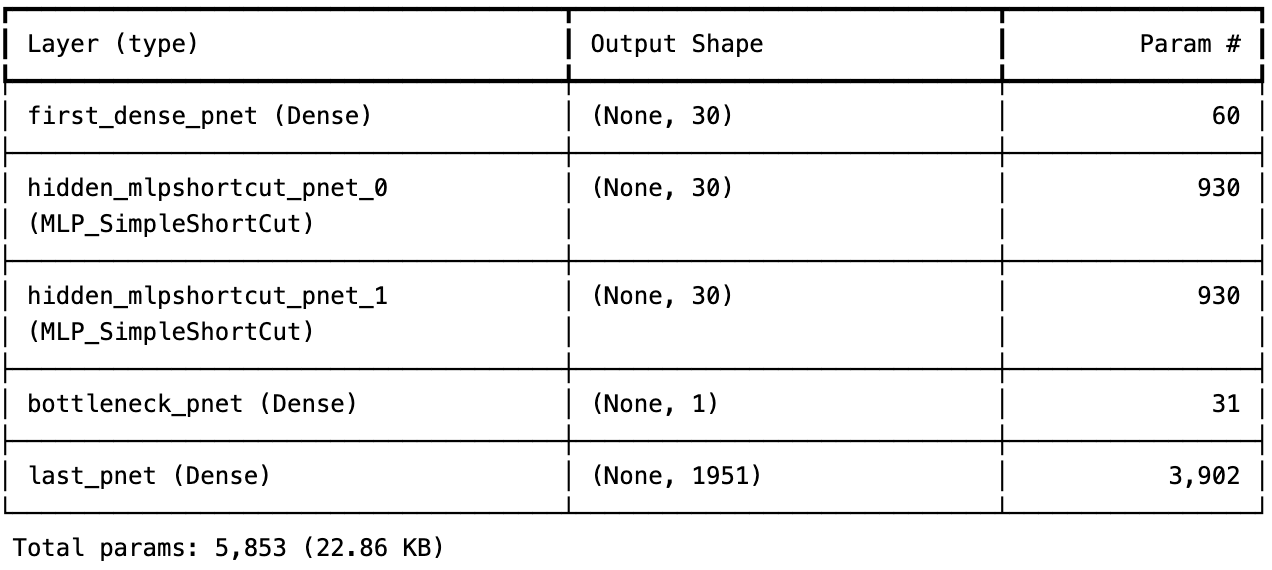
\includegraphics[width=\textwidth]{upstream-model.png}
        \caption{Upstream Reference Model Summary}
    \end{figure}
\end{frame}

\begin{frame}{TensorFlow Functional API Implementation}
    \begin{itemize}
        \item Complete architectural redesign
        \item Key features:
        \begin{itemize}
            \item Utilises TensorFlow's functional API
            \item Custom SIREN kernel initialization
            \item Dynamic layer generation
        \end{itemize}
        \item Optimizations:
        \begin{itemize}
            \item Automatic shape inference and building
            \item TF Function decoration for performance
            \item Full ParameterNet output forwarded to all ShapeNet layers
        \end{itemize}
    \end{itemize}
\end{frame}

\begin{frame}{TensorFlow Functional API Architecture}
    % \begin{itemize}
    %     \item ParameterNet:
    %     \begin{itemize}
    %         \item Dense (30) $\rightarrow$ 60 params
    %         \item 2x Shortcut (30) $\rightarrow$ 930 each
    %         \item Bottleneck (1) $\rightarrow$ 31 params
    %         \item Output (1951) $\rightarrow$ 3,902 params
    %     \end{itemize}
    %     \item Total: 5,853 params (22.86 KB)
    %     \item ShapeNet:
    %     \begin{itemize}
    %         \item 4x HyperDense layers
    %         \item Parameters generated by ParameterNet
    %     \end{itemize}
    % \end{itemize}
    \begin{figure}
        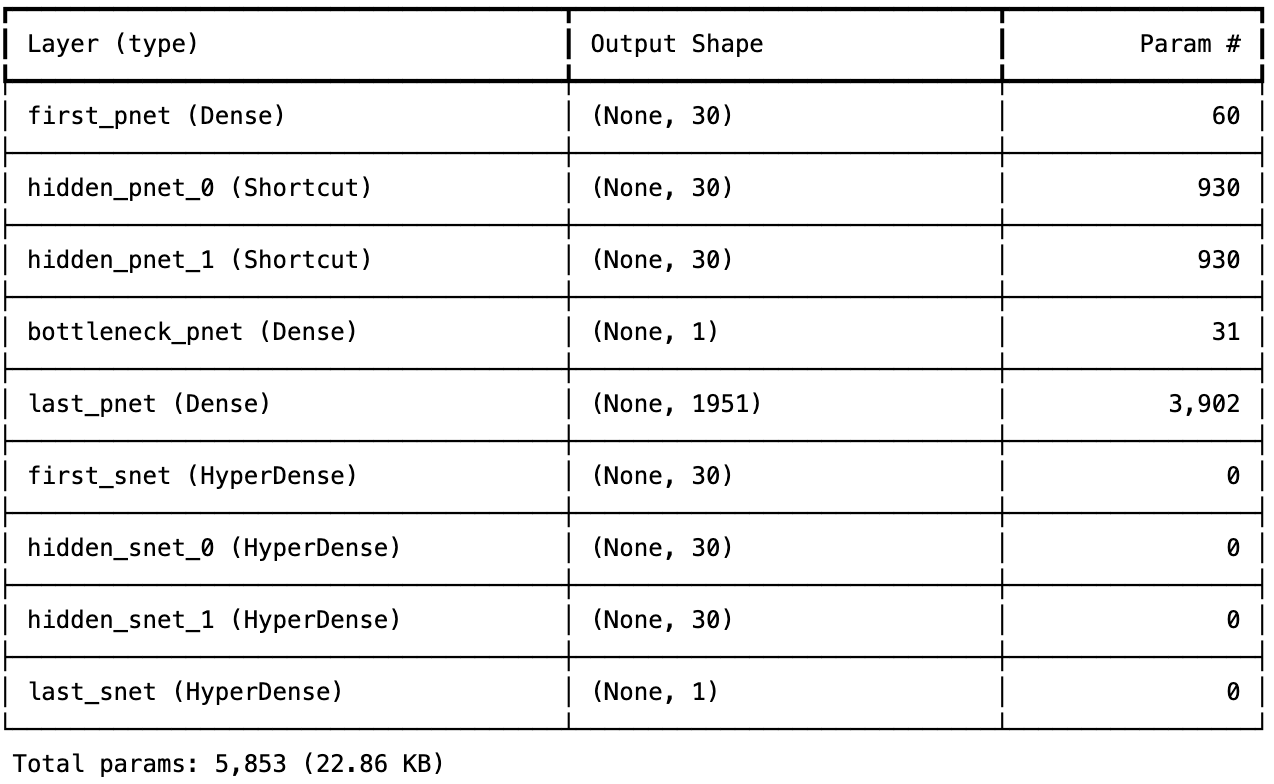
\includegraphics[width=0.8\textwidth]{functional-model.png}
        \caption{TensorFlow Functional API Model Summary}
    \end{figure}
\end{frame}

\begin{frame}{PyTorch Implementation}
    \begin{itemize}
        \item Core Features:
        \begin{itemize}
            \item Mixed precision training support (FP16/BF16)
            \item Custom StaticDense and StaticSIREN layers
            \item Gradient scaling and automatic mixed precision (AMP)
        \end{itemize}
        \item Implementation Details:
        \begin{itemize}
            \item Custom AdaBelief optimizer with gradient centralization
            \item Configurable learning rate scheduler with warmup
            \item Dynamic device handling (CPU/GPU) with dtype management
        \end{itemize}
        % \item Network Components:
        % \begin{itemize}
        %     \item ResNet and Shortcut layer implementations
        %     \item Flexible activation function mapping
        %     \item Parameter sharing through static layers
        % \end{itemize}
    \end{itemize}
\end{frame}

\begin{frame}{Test Cases}
    \begin{columns}
        \column{0.5\textwidth}
        \textbf{Low Frequency Traveling Wave}
        \begin{itemize}
            \item Domain: $x \in [0,1]$, $t \in [0,100]$
            \item 200 spatial points, 10 timesteps
            \item Simple periodic traveling wave
            \item $u(x,t) = \exp(-1000(x-x_0-ct)^2)$
        \end{itemize}
    
        \column{0.5\textwidth}
    \begin{figure}
        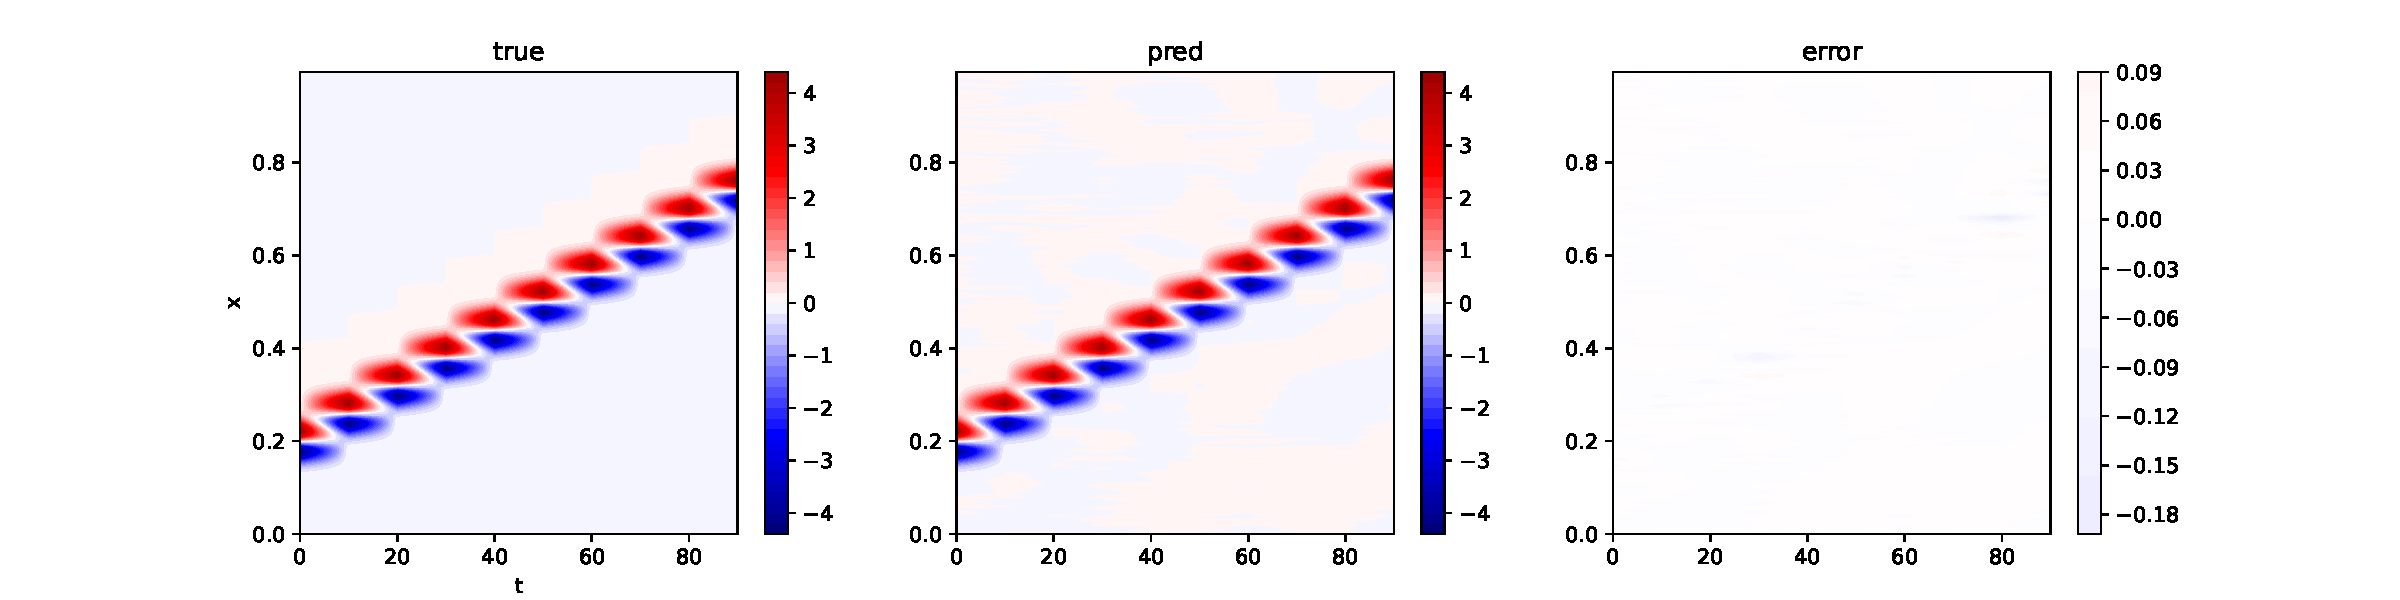
\includegraphics[width=0.85\textwidth,viewport=0 0 400 300,clip]{functional/low-frequency-adam-20250206-1105-1/vis}
            \caption{Low Frequency Example}
        \end{figure}
    \end{columns}
\end{frame}

\begin{frame}{Test Cases}
    \begin{columns}
        \column{0.5\textwidth}
        \textbf{High Frequency Traveling Wave}
        \begin{itemize}
            \item Same spatial/temporal domain
            \item Added frequency $\omega = 400$
            \item Complex oscillatory pattern
            \item $u(x,t) = \exp(-1000(x-x_0-ct)^2)\sin(\omega(x-x_0-ct))$
        \end{itemize}
        
        \column{0.5\textwidth}
        \begin{figure}
            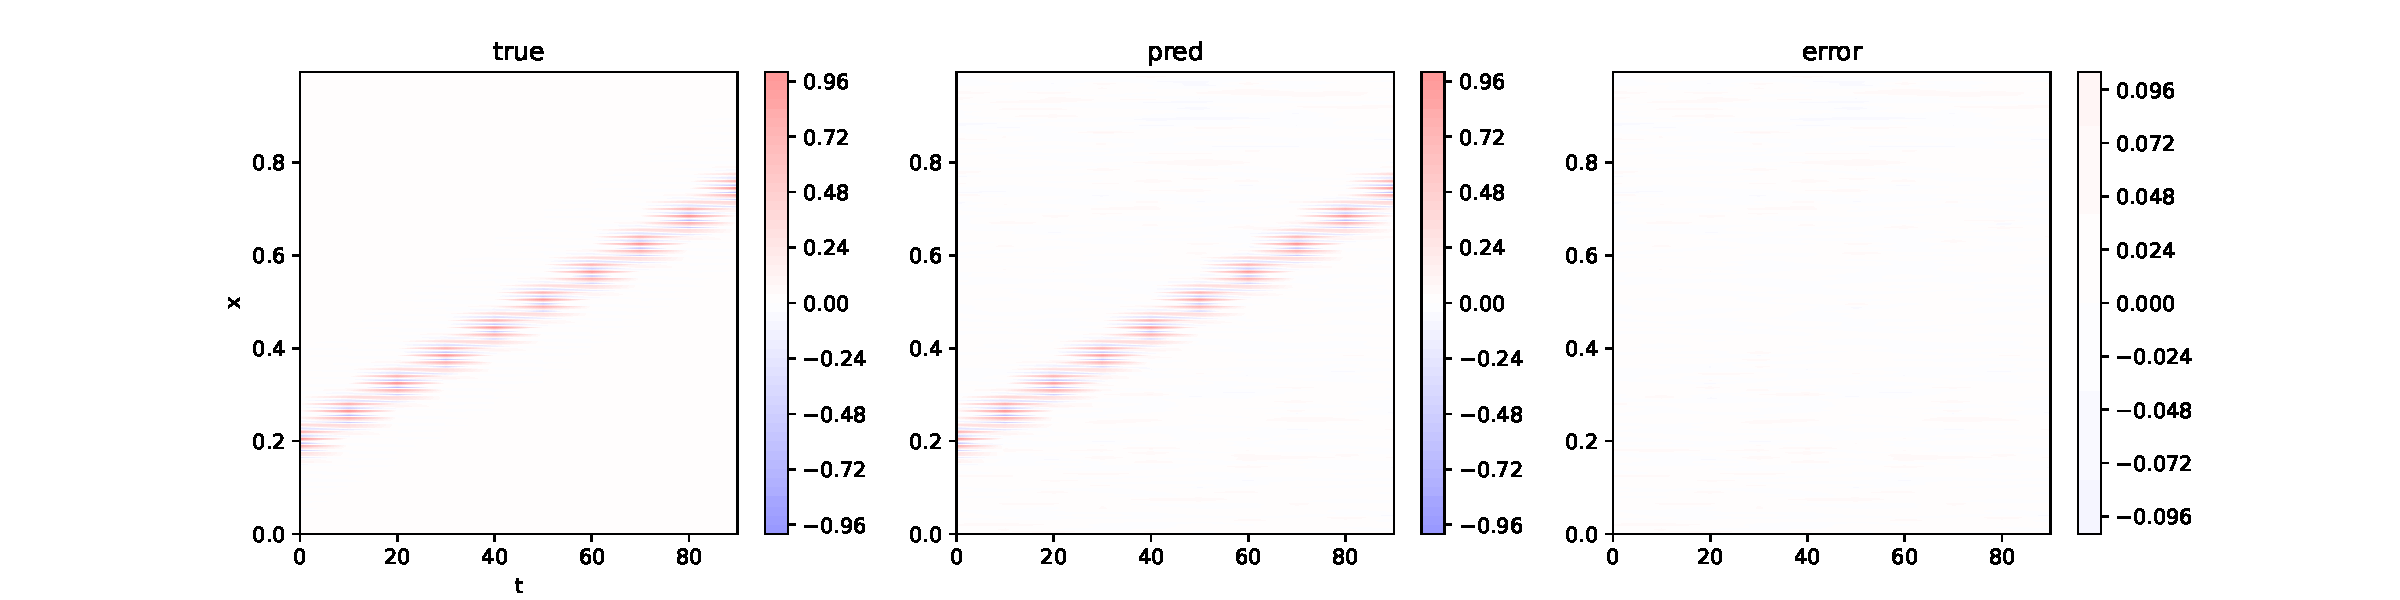
\includegraphics[width=0.85\textwidth,viewport=0 0 400 300,clip]{functional/high-frequency-adam-20250206-1520-1/vis}
            \caption{High Frequency Example}
        \end{figure}
    \end{columns}
\end{frame}

\begin{frame}{Network Architectures}
    \begin{columns}
        \column{0.5\textwidth}
        \textbf{ParameterNet}
        \begin{itemize}
            \item Dense input layer
            \item Two hidden layers (30 units)
            \item Bottleneck layer (1 unit)
            \item Adaptive output layer
        \end{itemize}
        
        \column{0.5\textwidth}
        \textbf{ShapeNet Variants}
        \begin{itemize}
            \item Shortcut (Low frequency)
            \begin{itemize}
                \item Skip connections
                \item Swish activation
            \end{itemize}
            \item SIREN (High frequency)
            \begin{itemize}
                \item Sinusoidal activation
                \item $\omega_0 = 30$ scaling
            \end{itemize}
        \end{itemize}
    \end{columns}
\end{frame}

\section{Results and Analysis}
\begin{frame}{Performance Overview}
    % \begin{columns}
    %     \column{0.5\textwidth}
    %     \begin{itemize}
    %         \item Low Frequency Best Result:
    %         \begin{itemize}
    %             \item Func. API: 1.526e-04
    %             \item PyTorch: 1.549e-04
    %             \item Upstream: 5.073e-04
    %         \end{itemize}
    %         \item High Frequency Best Result:
    %         \begin{itemize}
    %             \item PyTorch: 1.884e-04
    %             \item Func. API: 5.415e-04
    %             \item Upstream: N/A
    %         \end{itemize}
    %     \end{itemize}
        
    %     \column{0.5\textwidth}
        \begin{tikzpicture}[scale=1]
            \begin{axis}[
                ybar,
                bar width=0.4cm,
                width=0.8\textwidth,
                height=0.6\textheight,
                symbolic x coords={Low Freq.,High Freq.},
                enlarge x limits={abs=5*\pgfplotbarwidth},
                xtick=data,
                ymode=log,
                log origin=infty,
                ymin=1e-4,
                ymax=5e-3,
                ylabel={MSE Loss (log scale)},
                legend style={
                    at={(0.5,-0.25)},
                    anchor=north,
                    font=\tiny,
                    cells={anchor=west}
                },
                legend columns=2,
                ymajorgrids=true,
                grid style=dashed,
                nodes near coords style={
                    rotate=90,
                    anchor=west,
                    font=\tiny
                }
            ]
                % TF Functional API with Adam
                \addplot coordinates {
                    (Low Freq., 1.526e-4)
                    (High Freq., 5.415e-4)
                };
                % TF Functional API with AdaBelief
                \addplot coordinates {
                    (Low Freq., 2.487e-4)
                    (High Freq., 6.117e-4)
                };
                % PyTorch with Adam
                \addplot coordinates {
                    (Low Freq., 1.549e-4)
                    (High Freq., 1.884e-4)
                };
                % PyTorch with AdaBelief
                \addplot coordinates {
                    (Low Freq., 7.904e-4)
                    (High Freq., 2.219e-3)
                };
                % Upstream with Adam
                \addplot coordinates {
                    (Low Freq., 7.288e-4)
                    (High Freq., 0)
                };
                % Upstream with AdaBelief
                \addplot coordinates {
                    (Low Freq., 5.073e-4)
                    (High Freq., 0)
                };
                \legend{
                    TF Functional (Adam),
                    TF Functional (AdaBelief),
                    PyTorch (Adam),
                    PyTorch (AdaBelief),
                    Upstream (Adam),
                    Upstream (AdaBelief)
                }
            \end{axis}
        \end{tikzpicture}
    % \end{columns}
\end{frame}

% \begin{frame}{Processing Speed Comparison}
%     \begin{table}
%         \centering
%         \begin{tabular}{lcc}
%             \hline
%             \textbf{Implementation} & \textbf{Low Freq.} & \textbf{High Freq.} \\
%             \hline
%             TF Functional & 11.5-17K pts/s & 11.5-16K pts/s \\
%             PyTorch & 12-15K pts/s & 6-16K pts/s \\
%             Upstream & 12-17K pts/s & - \\
%             \hline
%         \end{tabular}
%         \caption{Processing Speed (points per second)}
%     \end{table}
% \end{frame}

\begin{frame}{Optimizer Impact}
    \begin{itemize}
        \item Adam vs AdaBelief comparison:
        \begin{itemize}
            \item TF Functional API: 62.5\% improvement
            \item PyTorch: 5.10x improvement (low freq.)
            \item PyTorch: 11.77x improvement (high freq.)
        \end{itemize}
        \item Key findings:
        \begin{itemize}
            \item Adam: More stable convergence
            \item Better final loss values
            \item Consistent across implementations
        \end{itemize}
    \end{itemize}
\end{frame}

\begin{frame}{Visual Results - Low Frequency}
    \begin{figure}
        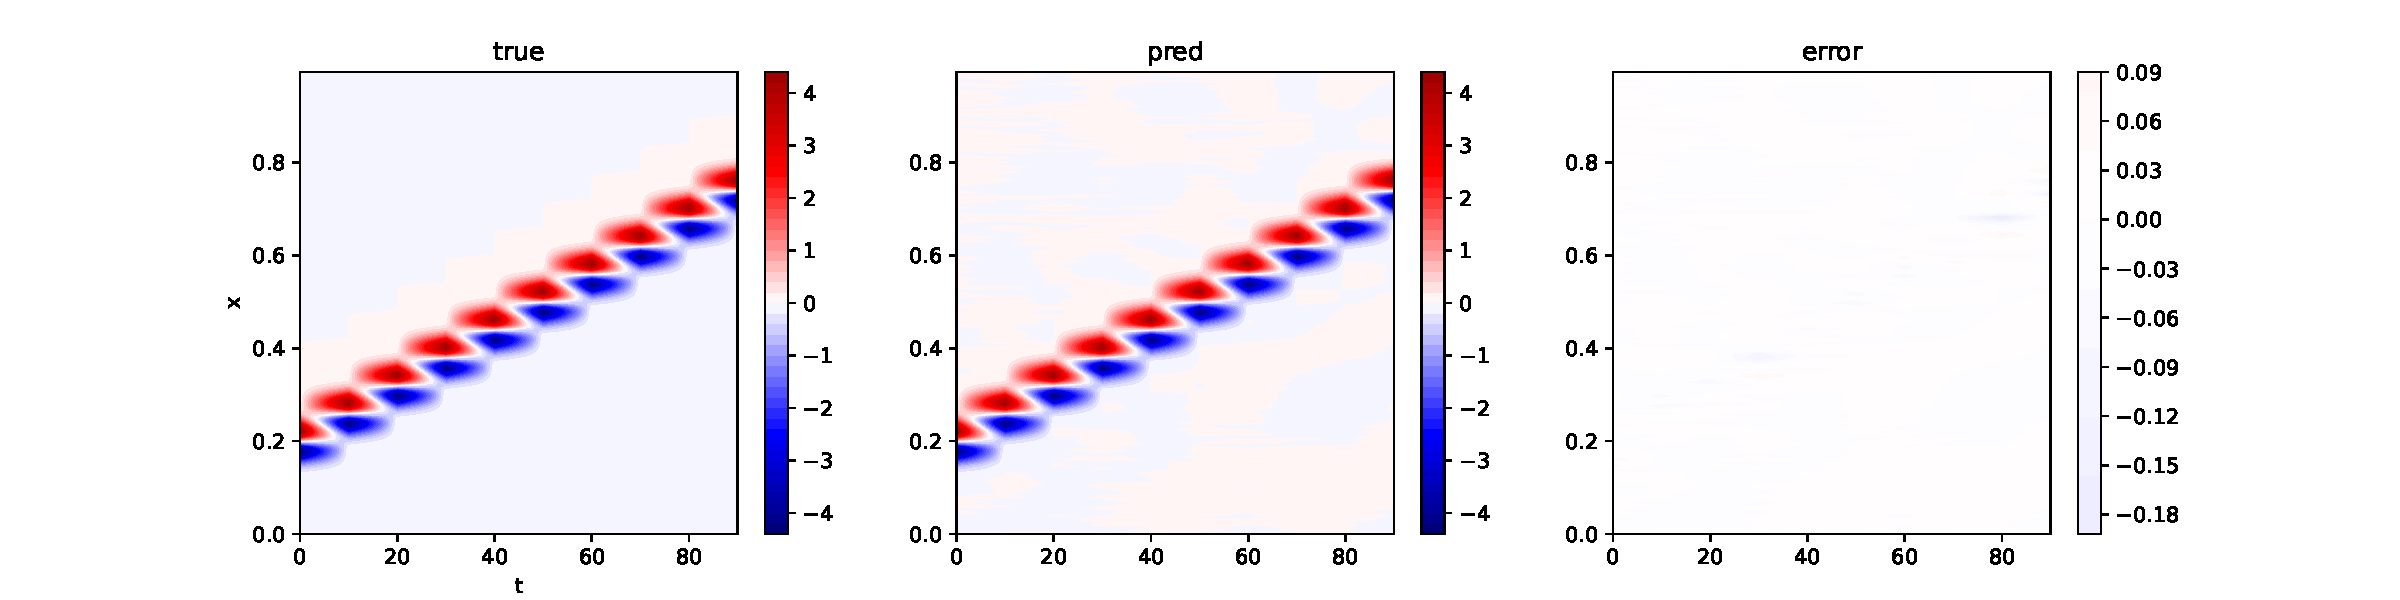
\includegraphics[width=\textwidth]{functional/low-frequency-adam-20250206-1105-1/vis}
        \caption{Low Frequency Predictions (TF Functional API)}
    \end{figure}
\end{frame}

\begin{frame}{Visual Results - High Frequency}
    \begin{figure}
        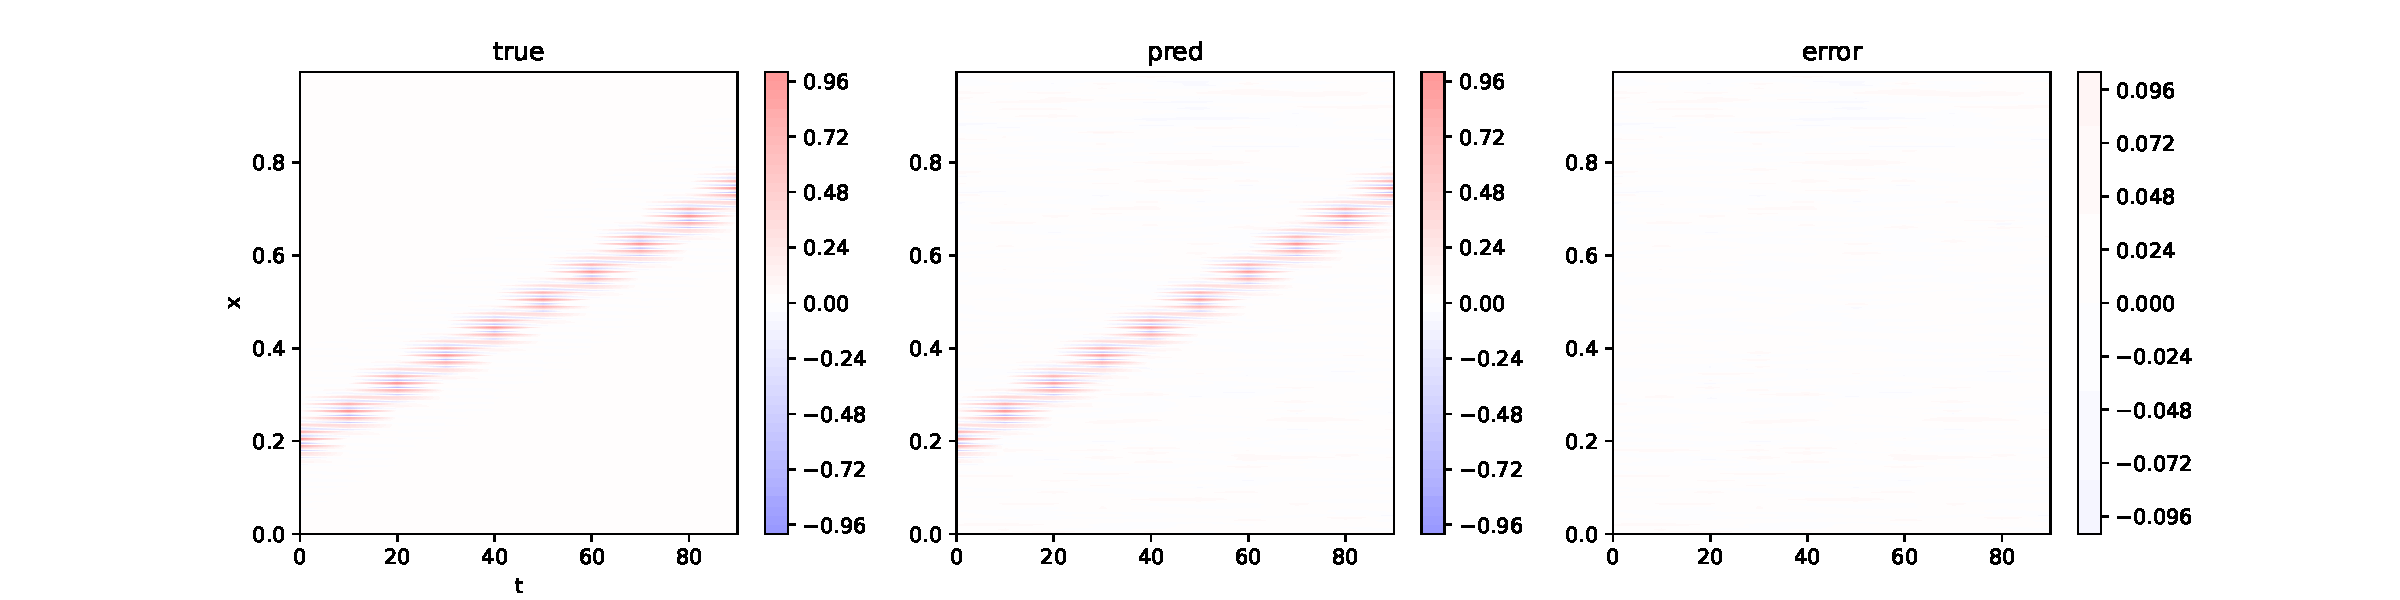
\includegraphics[width=\textwidth]{functional/high-frequency-adam-20250206-1520-1/vis}
        \caption{High Frequency Predictions (TF Functional API)}
    \end{figure}
\end{frame}

\section{Conclusions}
\begin{frame}{Key Findings}
    \begin{itemize}
        \item Implementation Trade-offs:
        \begin{itemize}
            \item Modern implementations have consistent performance
            \item PyTorch: Best high-frequency accuracy
        \end{itemize}
        \item Practical Implications:
        \begin{itemize}
            \item All implementations achieve production-ready speed
            \item Adam optimizer consistently outperforms AdaBelief
            % \item Framework choice impacts development experience
        \end{itemize}
    \end{itemize}
\end{frame}

% \begin{frame}{Future Directions}
%     \begin{itemize}
%         \item Technical Improvements:
%         \begin{itemize}
%             \item Additional network architectures
%             \item Memory optimization
%             \item Computational efficiency
%         \end{itemize}
%         \item Application Areas:
%         \begin{itemize}
%             \item Fluid dynamics
%             \item Climate modeling
%             \item Materials science
%         \end{itemize}
%         \item Research Opportunities:
%         \begin{itemize}
%             \item Complex spatio-temporal problems
%             \item Multi-scale phenomena
%             \item Real-time applications
%         \end{itemize}
%     \end{itemize}
% \end{frame}

\begin{frame}{Planned vs Achieved Goals}
    \begin{itemize}
        \item[\checkmark] Port from TensorFlow to PyTorch
        \item[+] Add TensorFlow Functional API implementation
        \item[\checkmark] Implement using upstream SIREN
        \item[\checkmark] Improve parallelism in training phase
        \item[$\times$] Compare to other HyperNetworks / LoRA / etc
        \item[\checkmark] Compare existing results with own implementation
        \item[$\times$] Compare performance with very hard example (e.g. weather prediction)
    \end{itemize}
\end{frame}


\begin{frame}
    \centering
    \Huge Thank you for your attention!
    
    \vspace{1cm}
    \Large Questions?
\end{frame}

\end{document}
